\section{The Worldwide LHC Computing Grid}
\label{wlcg}

The Worldwide LHC Computing Grid (WLCG) \cite{bird2011computing} is a global collaboration that links up more than 170 computing centers in 42 countries, serving an audience of more than 12000 physicists all around the world. 
As of 2022, WLCG constitutes the largest computing grid in the world and it is supported by many associated national and international grids, such as the European Grid Initiative and the Open Science Grid, as well as many other regional grids.
Founded in 2002 by CERN, the WLCG mission is to provide computing resources to store, distribute and analyze the data generated by the Large Hadron Collider.

Given the scale and complexity of the LHC data, this requires massive storage facilities, immense computing power, global networking, tailored software, adequate personpower and, of course, funding.
In order to achieve such challenging goals, WLCG leverages a distributed computing paradigm, where resources are shared among member states and made equally available to all the partners, regardless of their physical location.
% In brief, WLCG guarantees a seamless access to computing resources which include data storage capacity, processing power, sensors, and visualization tools, the resources that are capable to process over two million tasks daily, leveraging over one million computer cores and 1 exabyte of storage \cite{opint2022}.
\begin{figure}
    \centering
    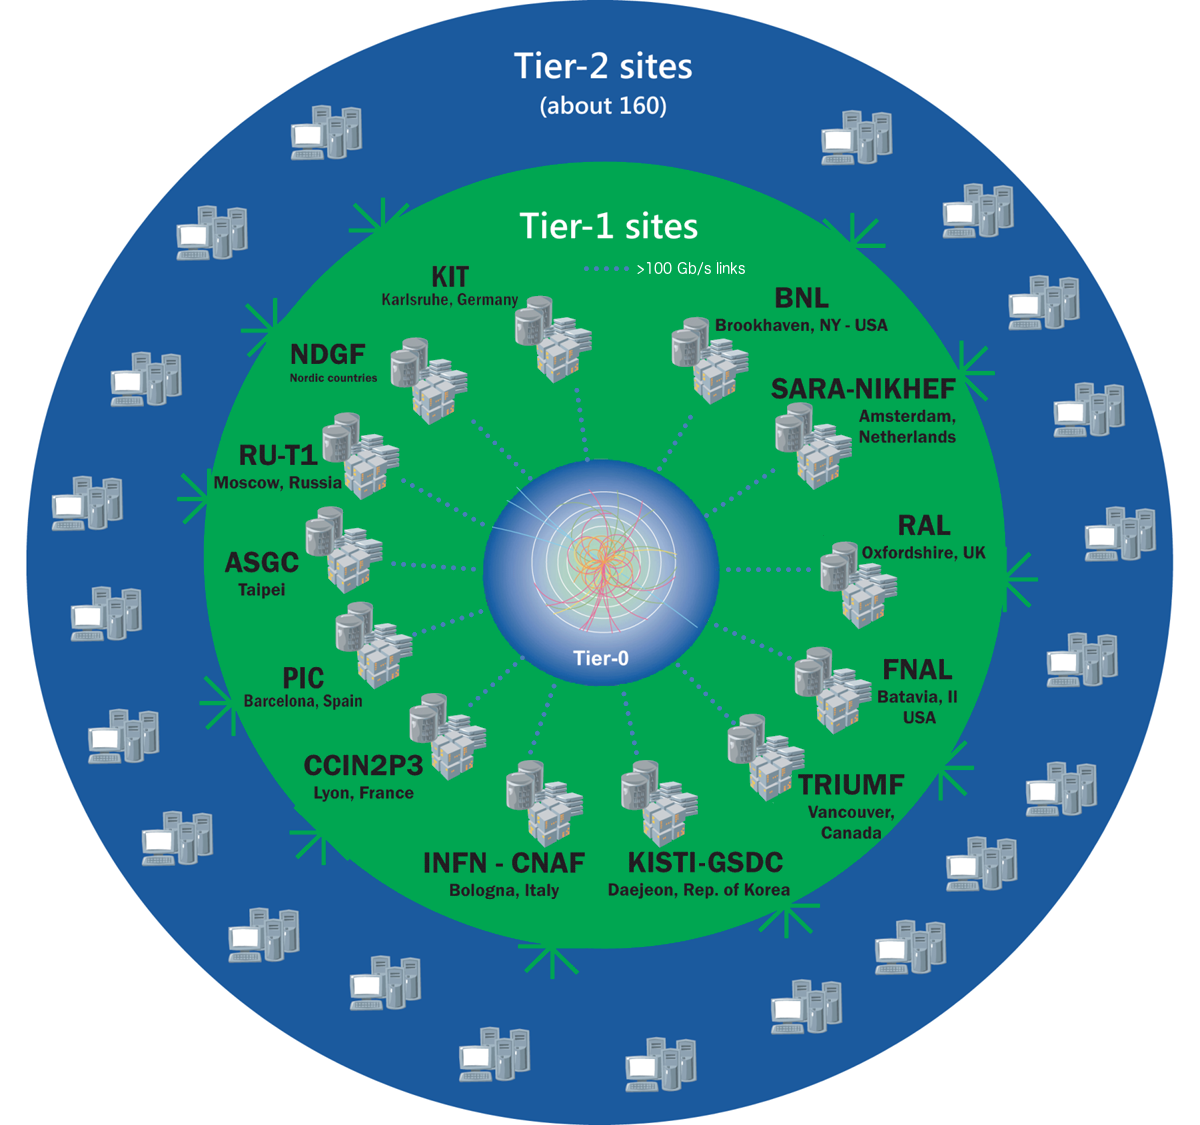
\includegraphics[width=\textwidth]{figures/220_introduction/WLCG-Tiers-2021_v3.png}
    \caption{\textbf{WLCG structure.} The Worldwide Large Hadron Collider Grid has a tiered structure organized into 4 levels and comprising more than 170 computing centers spread across 42 countries.
    } \label{fig:wlcg}
\end{figure}
\Cref{fig:wlcg} summarizes the WLCG infastructure composition. 
The Worldwide Large Hadron Collider Grid is structured in 4 levels, called \textit{tiers}, differing in terms of computing resources, storage capabilities and delivered services. 
% Proceeding from the bottom of this architecture, each layer sees an increased number
Its bottom layers comprise a few computing centers having great amounts of storage and processing resources, ultra-fast network connectivity (up to 100 GB/s), and they are devoted to general processing tasks.
The shallower layers, instead, group many smaller data centers devoted to more specialized activities.
In particular, the CERN data center is located at the bottom of this infrastructure, constituting the cornerstone of the whole architecture. 
It is located in Geneve (Switzerland) and it is endowed with more than 73000 processor cores, providing around 20\% of the total compute capacity of WLCG.
In terms of activity, the Tier-0 is responsible for i) the management of the raw data streams coming from the LHC experiments and their archiving for safe-keeping, ii) the reconstruction of physical entities like particles energy and velocity starting from the raw read-outs recorded by the electronic equipment, and iii) the distribution of raw and reconstructed data to the next tier layers.
Moving up the WLCG architecture, we find 13 large computer centres of the \textit{Tier-1s}.
These are directly linked to the Tier-0 and contribute to WLCG operations with sufficient storage capacity and round-the-clock support for the users. They are responsible for i) the safe-keeping of a proportional share of raw and reconstructed data, ii) large-scale reprocessing and safe-keeping of corresponding output, iii) access and distribution of data to the next infrastructure levels, and iv) safe-keeping of Monte Carlo simulated data.
One of these Tier-1 sites is located in Bologna\footnote{\cnaf} and it represents one of the biggest data centers in Italy. Its facilities count 40000 CPU cores, 40 PB of disk storage, 90 PB of tape storage, and the center is connected to the Italian (GARR) and European (GEANT) research network infrastructure with more than 200 Gbps \cite{cnaf2019annualrep, dell2019cnaf}.
The subsequent layer involves around 160 \textit{Tier-2} sites. These are data centers offered by universities and other scientific institutes, which are connected 
% to some of the Tier-1 sites 
through regional networks. 
They essentially act as analysis facilities to perform specialized tasks as the experiments production jobs and the Monte Carlo simulated data, which are then either stored locally or shared across the infrastructure.
% Despite having storage resources, the Tier-2s are not required to archive data, so the outputs produced there are typically sent back to Tier-1s when they are intended to be shared (as in the case of Monte Carlo data).
Finally, the last rung of the ladder is constituted by \textit{Tier-3s}. These sites enormously vary in scale,  ranging from local computing resources like university clusters or even individual pc to large national analysis facilities.
In fact, they do not formally belong to the WLCG but solely serve as entry points to its infrastructure for end-users analyses.

Alongside the hardware facilities, the WLCG supplies also advanced software solutions to provide researchers with seamless access to resources in a transparent way, without needing to worry about where the computing resources are coming from or where the data are physically stored.
This means that users can request access to data or resources from one of the many entry points into the system, and the grid infrastructure will then take care of spawning all the needed processes under the hood.
This may entail establishing the user identity and its access rights to the various sources, checking their credentials, and searching for available sites that can provide the requested resources.